\documentclass{article}
\usepackage[utf8]{inputenc}
\usepackage[spanish]{babel}
\usepackage{listings}
\usepackage{graphicx}
\graphicspath{ {Images/} }
\usepackage{cite}

\begin{document}

\begin{titlepage}
    \begin{center}
        \vspace*{1cm}
            
        \Huge
        \textbf{Informe Escrito}
            
        \vspace{0.5cm}
        \LARGE
        Parcial 2 - Segunda parte
            
        \vspace{1.5cm}
            
        \textbf{Julian Taborda Ramirez}
        
        \vspace{0.5cm}
        
        \textbf{Samuel Ruiz Vargas}
            
        \vfill
            
        \vspace{0.8cm}
            
        \Large
        Informatica II\\
        Universidad de Antioquia\\
        Medellín\\
        Septiembre de 2021
            
    \end{center}
\end{titlepage}

\tableofcontents
\vspace*{1.2cm}

\newpage

\section{Clases Implementadas}
\label{clases}

    \begin{flushleft}

    \end{flushleft}

    
\section{Esquema de las Clases}
\label{esquema}
    \begin{flushleft}

    \end{flushleft}
        
    
\section{Interacción de las Clases}
\label{interacciones}
    \begin{flushleft}
    
    \end{flushleft}
    
    
\section{Estructura del Circuito}
\label{circuito}
    \vspace{0.1cm}

    \begin{flushleft}
        \subsection{22/09}
        Iniciamos con una estructura simple que consta de un Arduino uno R3 conectado a una matriz de leds formada por 11 tiras de 16 Neopixeles; Para ello conectamos el puerto digital 2, 5V y GND a la primera tira de Neopixel, posteriormente conectamos las salidas de dicha tira con la siguiente tira y repetimos este proceso con todas las tiras de Neopixel.
    \end{flushleft}
    
    \begin{flushleft}
        \subsection{23/09}
        Actualizamos la matriz de leds a una 16x16, esto debido a que queremos que la matriz sea lo más fácil de tratar posible.
    \end{flushleft}
    
    \begin{figure}[h]
    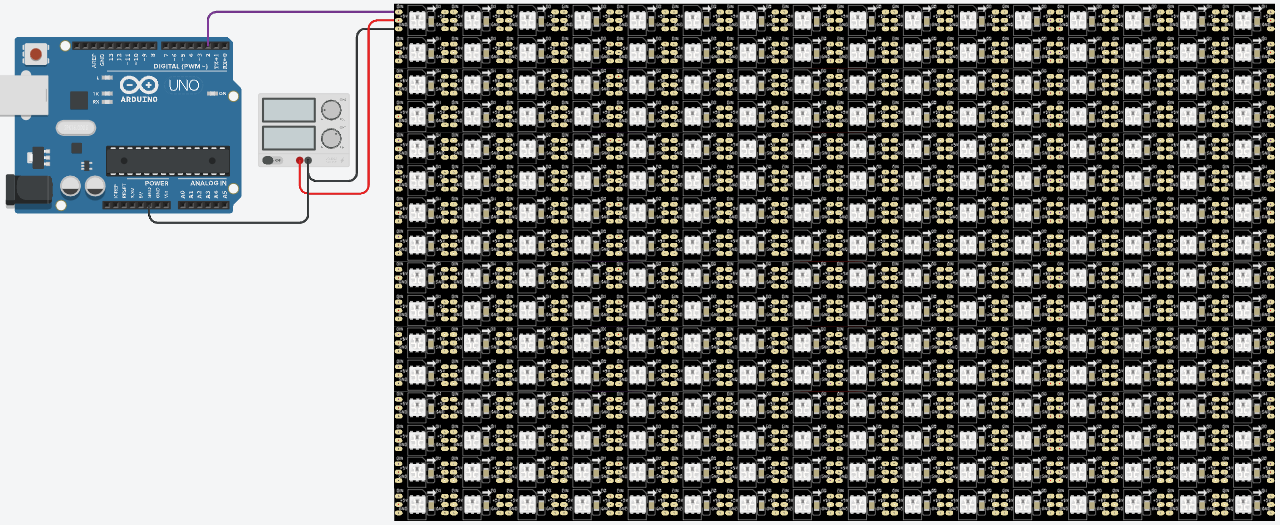
\includegraphics[width=12cm]{Images/leds.png}
    \centering
    \label{fig:leds}
    \end{figure}
    \vspace{0.5cm}
    
\section{Problemas Presentados}
\label{problemas}
    \begin{flushleft}
     \subsection{23/09}
     En este día, luego de plantear el código en QT, nos encontramos con la siguientes problematicas:
    \end{flushleft}
    
    \begin{flushleft}
    \subsubsection{Muestreos}
    Hasta el momento no hemos evaluado la técnica necesaria para realizar un submuestreo o sobremuestro según la imagen elegida, como su vez no hemos implementado la carga respectiva de la imagen.  
    \end{flushleft}
    
    \begin{flushleft}
    \subsubsection{Retorno de informacion}
    Para esta parte del programa, aún no tenemos muy claro como vamos a entregar la información requerida por Tinkercad de tal manera que se adapte a la representación de la matriz.  
    \end{flushleft}
    
    \begin{flushleft}
     \subsection{24/09}
     En este día realizamos la parte más sencilla del código que es sacar los datos de la imagen original, nos topamos con el problema de que no podíamos introducir todos los datos en una sola matriz, puesto que en algunos casos hay demasiada información, por lo que decidimos separar los datos en 3 arreglos, uno para los rojos, otro para los verdes y el último para los azules.
    \end{flushleft}
    
\section{Manual de Uso Rápido}
\label{manual}
    \begin{flushleft}
        
    \end{flushleft}

\vfill
\bibliographystyle{IEEEtran}


\end{document}
